%% LyX 2.0.3 created this file.  For more info, see http://www.lyx.org/.
%% Do not edit unless you really know what you are doing.
\documentclass{article}
\usepackage[latin9]{inputenc}
\usepackage{graphicx}

\makeatletter
%%%%%%%%%%%%%%%%%%%%%%%%%%%%%% User specified LaTeX commands.


\usepackage{array}\usepackage{rotating}




\providecommand{\tabularnewline}{\\}





\makeatother

\begin{document}

\section{Introduction}

User`s space database is separate part of database. Contains all data,
which are used in comunication between user and server.


\section{Logic Structure}

User space database contains information about user and documents,
which are uploaded by him. User database objects are User, Document
, TranslationResult , TranslationPair , Session. Relations beetwen
them are very simple. First part is for authentication contains objects
User and Session. User object is created by registration and this
object are peristent, but changeable (password, email ...) by user.
Session object is assigned each user after log in. Session contains
session key (is possible get userId from session key) according it
can be traceable user and his statistics. Session object is not changeable
by user. Rest objects (Document,TranslationResult,TranslationPair)
reprezents relation between user and documents, that are uploaded
by user. It is obvious according name, that documents can contains
n translation result. Translation result is in fact selected one from
offered possibilities represented by TranslationPair object.


\section{Physical Structure}

Userspace database is quite simple. Each object described above have
own table. Accordnig relationship between objects contains tables
with Documents, TranslationResult ,TranslationPair foreign keys from
connected tables. Better picture about relations between tables can
be provided by image below. 
\begin{figure}
\begin{centering}
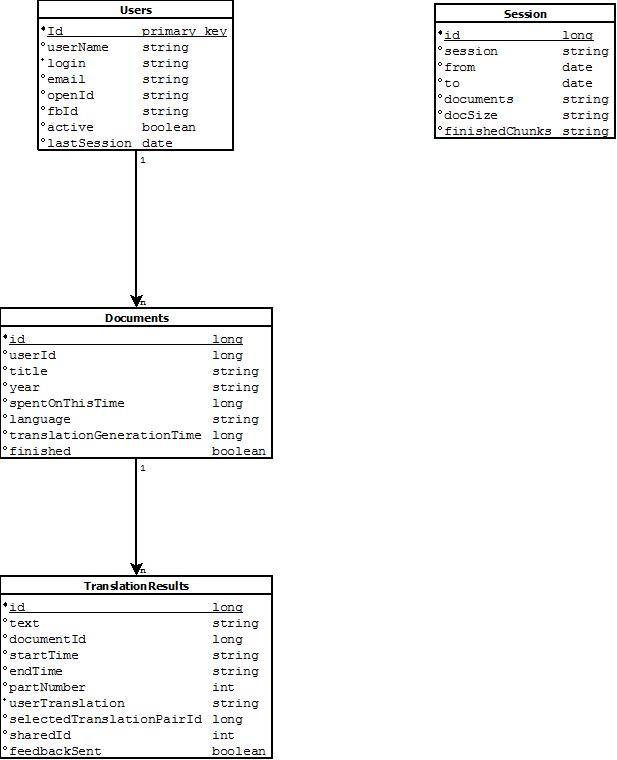
\includegraphics{Userspace.jpeg} 
\par\end{centering}

\caption{Design of userspace database}
\end{figure}

\end{document}
